\documentclass[preprint,11pt]{elsarticle}
\usepackage[margin=2.5cm]{geometry}
\usepackage{gensymb,amsmath,amsfonts,amssymb,float,enumerate}
\usepackage{graphicx,multicol,bm,subcaption}
\usepackage{subdepth}
\usepackage{multirow}
\usepackage{makecell}
\usepackage{hyperref}
\usepackage{algorithm}
\usepackage{algpseudocode}
\usepackage[ruled,noline,noend]{algorithm2e}
\usepackage{csquotes}
\hypersetup{
    colorlinks=true,       % false: boxed links; true: colored links
    linkcolor=blue,        % color of internal links (sections, etc.)
    citecolor=green,       % color of citation links
    filecolor=magenta,     % color of file links
    urlcolor=cyan          % color of external links
}
\usepackage{lipsum}
% \usepackage{biblatex}
\title{
    % \vspace{-1em}  % Adjust space before the line
    \hrule height 1.5pt  % Upper bold line
    \vspace{0.5em}  % Space between line and title
    {\Large GP-Tree: A Gaussian Process Classifier for Few-Shot Incremental Learning}  % Title text
    \vspace{0.5em}  % Space between title and line
    \hrule height 1.5pt  % Lower bold line
    % \vspace{1em}  % Adjust space after the line
}
\journal{$\mathit{38}^{th}$ International Conference on Machine Learning,PMLR 139, 2021}
\begin{document}

% \title{GP-Tree: A Gaussian Process Classifier for Few-Shot Incremental Learning\tnoteref{}}

% \author[inst1]{Idan Achituve}
% \ead{idan.achituve@biu.ac.il}
% \author[biu]{Idan Achituve\corref{idan}}
% \author[biu]{Aviv Navon}
% \author[biu]{Yochai Yemini}
% \author[biu,nvidia]{Gal Chechik}
% \author[biu]{Ethan Fetaya}

\author[biu]{Idan Achituve}
\author[biu]{Aviv Navon}
\author[biu]{Yochai Yemini}
\author[]{Gal Chechik\textsuperscript{1 2}}
\author[biu]{Ethan Fetaya}


% \fntext[fn1]{Correspondence to: Idan Achituve $<$idan.achituve@biu.ac.il$>$.}
% Affiliations
% Corresponding author
% \cortext[cor1]{\textsuperscript{1}Bar-Ilan University,\textsuperscript{2}Nvidia}
% \begin{keyword}
% Gaussian Process Classification \sep Incremental Learning \sep Deep Kernel Learning
% \end{keyword}
% \tnotetext[t1]{Proceedings of the 38th International Conference on Machine Learning, PMLR 139, 2021. Copyright 2021 by the author(s).}
% \affiliation[inst1]{Department of Mathematics, University X}
% \affiliation[inst2]{Department of Biology, University Y}
% \fntext[label1,label2]{Bar-Illan University,\textsuperscript{2}Nvidia}

% \title{\LARGE\textbf{Bridge Girth: A Unifying Notion in Network Design}}

% \author[1]{Greg Bodwin}
% \ead{bodwin@umich.edu}

% \author[1]{Gary Hoppenworth}
% \ead{garytho@umich.edu}

% \author[2]{Ohad Trabelsi\corref{cor1}}
% \ead{ohadt@ttic.edu}

% \address[1]{Department of Electrical Engineering and Computer Science, University of Michigan, Ann Arbor, USA}
% \address[2]{Toyota Technological Institute at Chicago, Chicago, USA}

% \address[biu]{Bar-Ilan University}
% \address[nvidia]{Nvidia}
% \tnotetext[t1]{\textit{Proceedings of the $\mathit{38}^{th}$ International Conference on Machine
% Learning}, PMLR 139, 2021. Copyright 2021 by the author(s).}
% \cortext[idan]{Correspondance to: Idan Achituve $<$\href{mailto:idan.achituve@biu.ac.il}{idan.achituve@biu.ac.il}$>$}


\tnotetext[t1]{\textsuperscript{1}Bar-Ilan University \textsuperscript{2}Nvidia. Correspondence to: Idan Achituve $<$\href{mailto:idan.achituve@biu.ac.il}{idan.achituve@biu.ac.il}$>$}

% \cortext[cor2]{\textit{Proceedings of the $\mathit{38}^{th}$ International Conference on Machine Learning}, PMLR 139, 2021. Copyright 2021 by the author(s).}
\cortext[cor2]{Copyright 2021 by the author(s).}
\date{\today}
% \tableofcontents


\begin{abstract}
\label{abs}
Gaussian processes (GPs) are non-parametric,
flexible, models that work well in many tasks.
Combining GPs with deep learning methods via
deep kernel learning (DKL) is especially compelling
due to the strong representational power
induced by the network. However, inference in
GPs, whether with or without DKL, can be computationally
challenging on large datasets. Here,
we propose \textit{GP-Tree}, a novel method for multiclass
classification with Gaussian processes and
DKL.We develop a tree-based hierarchical model
in which each internal node of the tree fits a GP
to the data using the Pólya-Gamma augmentation
scheme. As a result, our method scales
well with both the number of classes and data
size. We demonstrate the effectiveness of our
method against other Gaussian process training
baselines, and we show how our \textit{general} GP approach
achieves improved accuracy on standard
incremental few-shot learning benchmarks.
\end{abstract}

%\begin{document}
\maketitle

% Pólya
\section{Introduction}
\label{sec:1}
This paper discusses Gaussian Processes (GPs), a Bayesian nonparametric approach, which, despite their advantages, face challenges in kernel selection and scalability, particularly in image domains. To address this, deep kernel learning (DKL) is used to improve kernel functions, but scalability issues arise when handling large datasets. The paper proposes a novel method, GP-Tree, for scalable Gaussian Process Classification (GPC), especially for multi-class problems. GP-Tree combines a tree-based model and the Pólya-Gamma augmentation, overcoming the limitations of prior GPC methods. Additionally, it demonstrates superior performance in incremental few-shot learning tasks, offering promising results.

% \vspace{1em}
% \noindent\rule{0.3\textwidth}{0.4pt}

% \noindent\textsuperscript{1}Bar-Ilan University \textsuperscript{2}Nvidia. Correspondence to: Idan Achituve $<$\href{mailto:idan.achituve@biu.ac.il}{idan.achituve@biu.ac.il}$>$

% \vspace{1em}

% \textit{Proceedings of the 38th International Conference on Machine Learning}, PMLR 139, 2021. Copyright 2021 by the author(s).






\section{Background}
\label{sec:2}
    \subsection{Notations}
    \label{sec:2.1}
        We denote vectors with bold lower-case font, e.g., $\boldsymbol{x}$, and matrices with capital bold font, e.g., $\bm{X}$. Given a dataset $(\boldsymbol{x}_1, y_1), \ldots, (\boldsymbol{x}_n, y_n)$, we denote by $\boldsymbol{y} = [y_1, \ldots, y_n]^T$ the vector of labels, and by $\bm{X} \in \mathbb{R}^{n \times d}$ the design matrix whose $i^{th}$ row is $\boldsymbol{x}_i$. In the classification case, each $y_i$ takes a value from $\{1, \ldots, C\}$ class labels.
    \subsection{Gaussian Processes}
    \label{sec:2.2}
        In Gaussian process learning we assume the mapping from
        the input points to the target values is via a latent function
        $f$.The target values are assumed to be independent
        when conditioned on the latent function, i.e., $p(\boldsymbol{y}|\bm{X},f)=\prod_{i=1}^{n}\, p(y_i|f(\boldsymbol{x_i}))$.The latent function is assumed to follow
        a Gaussian process prior $f\sim\mathcal{GP}\,(m(\boldsymbol{x}),k(\boldsymbol{x},\boldsymbol{x'}$)), where
        the evaluation vector of $f$ on $\bm{X}$, $\boldsymbol{f} = [f(x_1),\ldots,f(x_n]^T$ has a Gaussian distribution $\bm{f} \sim \mathcal{N}(\mu,\boldsymbol{K})$, where $\bm{\mu}_i = m(\bm{x_i})$ and $\bm{K}_{ij} = k(\bm{x_i},\bm{x_j}).$ The mean $m(\bm{x})$ is commonly taken to be the constant zero function, and the kernel
        $k(\bm{x},\bm{x'})$ is a positive semi-definite function.
        \\
        Let $\bm{X}$, $\bm{y}$ be the training data, and let $f_*$ be the evaluation
        of $f$ on a novel point $x_*$. In the regression case, we
        assume $p(y|\bm{x}, f) = \mathcal{N}(f(\bm{x}), \sigma^2)$. Therefore, the predictive distributions, $p(f_*|\bm{x}_*, \bm{y},\bm{X})$ and $p(y_*|\bm{x}_*, \bm{y},\bm{X}) = \int p(f_*|\bm(x)_*,\bm{y},\bm{X})p(y_*|f_*)df_* $, are Gaussians with known parameters. Specifically,
        \begin{align}
            &p( f_*|\bm{x}_*,\bm{y},\bm{X} = \mathcal{N}( \mu_*,\sigma_* ) ), \nonumber \\
            &\mu_*  = \bm{k}_*^T( \bm{K}+\sigma^2\bm{I} )^{-1}\bm{y}, \\
            &\sigma_* = k_{**} - \bm{k}_*^T( \bm{K} + \sigma^2I )^{-1}\bm{k}_*.\nonumber
        \end{align}
        Where, $k_{**} = k(x_*, x_*)$, and $\bm{k}_*[i] = k(\bm{x}_i; \bm{x}_*)$. This
        closed-form solution allows us to avoid the costly marginalization
        step; however, it entails the inversion of an $n \times n$
        matrix which can be expensive to compute for large datasets.\\
        \\
        %citation
        DKL (\textit{Wilson et al., 2016a}\cite{wilson2016deep}) is a popular choice to apply a
        kernel on structured data such as images. The kernel over the
        input data points is commonly in the form of a fixed kernel
        on an embedding learned by a deep neural network $g_\theta$, e.g.,
        $k_\theta(\bm{x}, \bm{x'}) = exp( -||g_\theta( \bm{x} ) - g_\theta(\bm{x'}||^2/2\ell^2)  )$. Therefore,
        the closed-form inference is of even greater importance as
        it allows to easily backpropagate through the GP inference.
        
    \subsection{The Pólya-Gamma Augmentation}
    \label{sec:2.3}
        %citation
        When applying GPs to classification tasks, the likelihood
        $p(y|f(\bm{x}_i))$ is no longer Gaussian. The predictive distributions
        are also no longer Gaussian and we do not have a
        close-form solution for them. To overcome this limitation,
        several methods were offered based on the Pólya-Gamma
        augmentation (\textit{Polson et al., 2013}\cite{polson2013bayesian}) to model the discrete
        likelihoods in GPs (\textit{Linderman et al., 2015}\cite{linderman2015dependent}; \textit{Wenzel et al.,
        2019}\cite{wenzel2019efficient}; \textit{Galy-Fajou et al., 2020}\cite{galy2020multiclass}; \textit{Snell \& Zemel, 2021}\cite{snell2021bayesian}). The
        Pólya-Gamma augmentation hinges on the following identity
            \begin{align}
                \frac{( e^\psi )^a}{(  1+e^\psi)^b} = 2^{-b}e^{\kappa \psi} \mathbb{E}_\omega[ e^{-\omega \psi^2 /2 } ]\,,
            \end{align}
        where $\kappa = a-b /2$ and $\omega$ has the Pólya-Gamma distribution $\omega \sim PG(b,0)$.
        \\
        Suppose we have a binary classification task with $y \in \{0, 1\}$, and we are given a vector of latent function values $\bm{f}$, the likelihood can be written as,
            \begin{align}
                p(\bm{y}|\bm{f}) = \prod_{j=1}^{n}|\sigma( f_i )^{y_i}( 1-\sigma(  f_i) )^{1-y_i} = \prod_{j=1}^{n} \frac{e^{y_i f_i}}{1+e^{f_i}},
            \end{align}
        \\
        where $\sigma(\cdot)$ is the sigmoid function. We can now use Eq. 2
        to introduce auxiliary Pólya-Gamma variables (one per sample)
        such that we recover Eq. 3 by marginalizing them out.
        If instead we sample the Pólya-Gamma variables $\bm{\omega}$ we get
        the following posteriors:
        \begin{equation}
            \begin{split}
                p( \bm{f}|\bm{y}, \bm{\omega} ) &= \mathcal{N}( \bm{f}|\Sigma(\bm{K}^{-1}\bm{\mu} + 1), \Sigma ), \\
                p( \bm{\omega}| \bm{y}, \bm{f} ) &= PG(\bm{1}, \bm{f}).
            \end{split}
        \end{equation}
        \\
        Where $\kappa_j = y_j- 1/2, \Sigma = (\bm{K}^{-1} + \bm{\Omega} )^{-1}$, and 
        $ \bm{\Omega}= diag(\bm{\omega})$. We can now sample from $p(\bm{f},\bm{\omega}|\bm{y},\bm{X})$ using
        block Gibbs sampling and get Monte-Carlo estimations of
        the marginal and predictive distributions.

    \subsection{Inducing Points}
    \label{sec:2.4}
        Exact inference with GPs compels us to store the entire
        training set and invert an $n \times n$ matrix $\bm{K}_{nn}$, which greatly
        limits their use. A common solution to this problem is to
        use inducing points (\textit{Silverman, 1985}\cite{silverman1985some}; \textit{Quinonero-Candela \& Rasmussen, 2005}
        \cite{quinonero2005unifying}; \textit{Snelson \& Ghahramani, 2006}\cite{snelson2006sparse}). With
        inducing points, we usually define $m \ll n $ pseudo-inputs
        whose locations are often trainable parameters. Then we
        only need to invert an $m \times m$ matrix, thus allowing us to
        control the computational cost.
        \\
        Our approach closely follows the inducing points method for
        binary classification with the Pólya-Gamma augmentation
        presented in (\textit{Wenzel et al., 2019}\cite{wenzel2019efficient}). We define $\bm{\Bar{X}}$
        as the
        inducing locations/inputs and $\bm{\Bar{X}}$ as the latent function value
        evaluated on $\bm{\Bar{X}}$. We have,
        \begin{equation}
            p(\bm{\Bar{f}}) = \mathcal{N}( 0,\bm{K}_{mm} ),\\
        \end{equation}
        \begin{equation}
            \begin{split}
                p(f|\bm{\Bar{f}}) = \mathcal{N}( \bm{K}_{nm}{\bm{K}}_{mm}^{-1}\Bar{\bm{f}},\bm{Q}_{nn} ),\\
                \bm{Q}_{nn} = \bm{K}_{nn} - \bm{K}_{nm}\bm{K}_{nm}^{-1}\bm{K}_{nm}.
            \end{split}
        \end{equation}
        \begin{equation}
            p( \bm{y},\bm{\omega},\bm{f},\bm{\Bar{f}} ) = p( \bm{y}|\bm{f},\omega )p( \bm{f}|\bm{\Bar{f}} )p( \bm{\Bar{f}} )p(\bm{\omega}),
        \end{equation}
        where $K_{mm}$ is the kernel matrix on the inducing locations,
        and $K_{nm}$ is the cross-kernel matrix between the inputs and
        the inducing locations. While $p(\bm{\Bar{f}}|y)$ is Gaussian due
        to the Pólya-Gamma augmentation, the distribution after
        marginalizing over $\bm{\omega}$, $p( \bm{\Bar{f}}|\bm{y} )$, is not Gaussian. Following
        (\textit{Hensman et al., 2015}\cite{hensman2015scalable}),\textit{Wenzel et al. (2019)}\cite{wenzel2019efficient} proposed a variational
        inference approach based on the following assumption
        $q(\bm{\omega}, \bm{\Bar{f}}) = q(\bm{\omega})q(\bm{\Bar{f}})$, where $q(\bm{\omega})$ is a Pólya-Gamma
        density and $q(\bm{\Bar{f}})$ is a Gaussian density. Then, the inducing
        locations and the variational parameters are learned with the
        evidence lower bound.
            
    \section{Method}
    \label{sec:3}
    In Sections \ref{sec:3.1}-\ref{sec:3.3} we describe our method to train GP
    classifiers with DKL that scale to large training sets and
    a large number of classes. Afterward, in Section \ref{sec:3.4}, we
    will show how our model, with minor modifications, can be
    adjusted to the few-shot class-incremental learning setup.
        \subsection{Hierarchical Classification}
        \label{sec:3.1}
        Consider the case presented in (\textit{Linderman et al., 2015}\cite{linderman2015dependent})
        aimed at modeling categorical and multinomial data. To derive
        a Pólya-Gamma augmentation \textit{Linderman et al. (2015)}\cite{linderman2015dependent}
        utilized the stick-breaking representation for the multinomial
        density. They turn the multi-class classification task
        into a sequence of $C - 1$ binary classification tasks where
        $y^j = 1$ if the original label is $j$ and $y^j = 0$ if the original
        label is larger than $j$. Then, $C - 1$ independent Gaussian
        processes can be learned, one for each of the binary classification
        tasks. Denoting by $\bm{f}_i = (f_i^1, \ldots , f_i^{C-1} )$ the vector of
        latent processes values at the $i^{th}$ example, the stick-break
        likelihood is:
        \begin{equation}
            p( y_i = c|\bm{f}_i ) = \sigma( f^c ) \prod_{k<c} ( 1-\sigma( f^k )  ),
        \end{equation}
        %image adding before proceeding
        \begin{figure}
            \centering
            \begin{subfigure}[b]{0.3\textwidth}
                \centering
                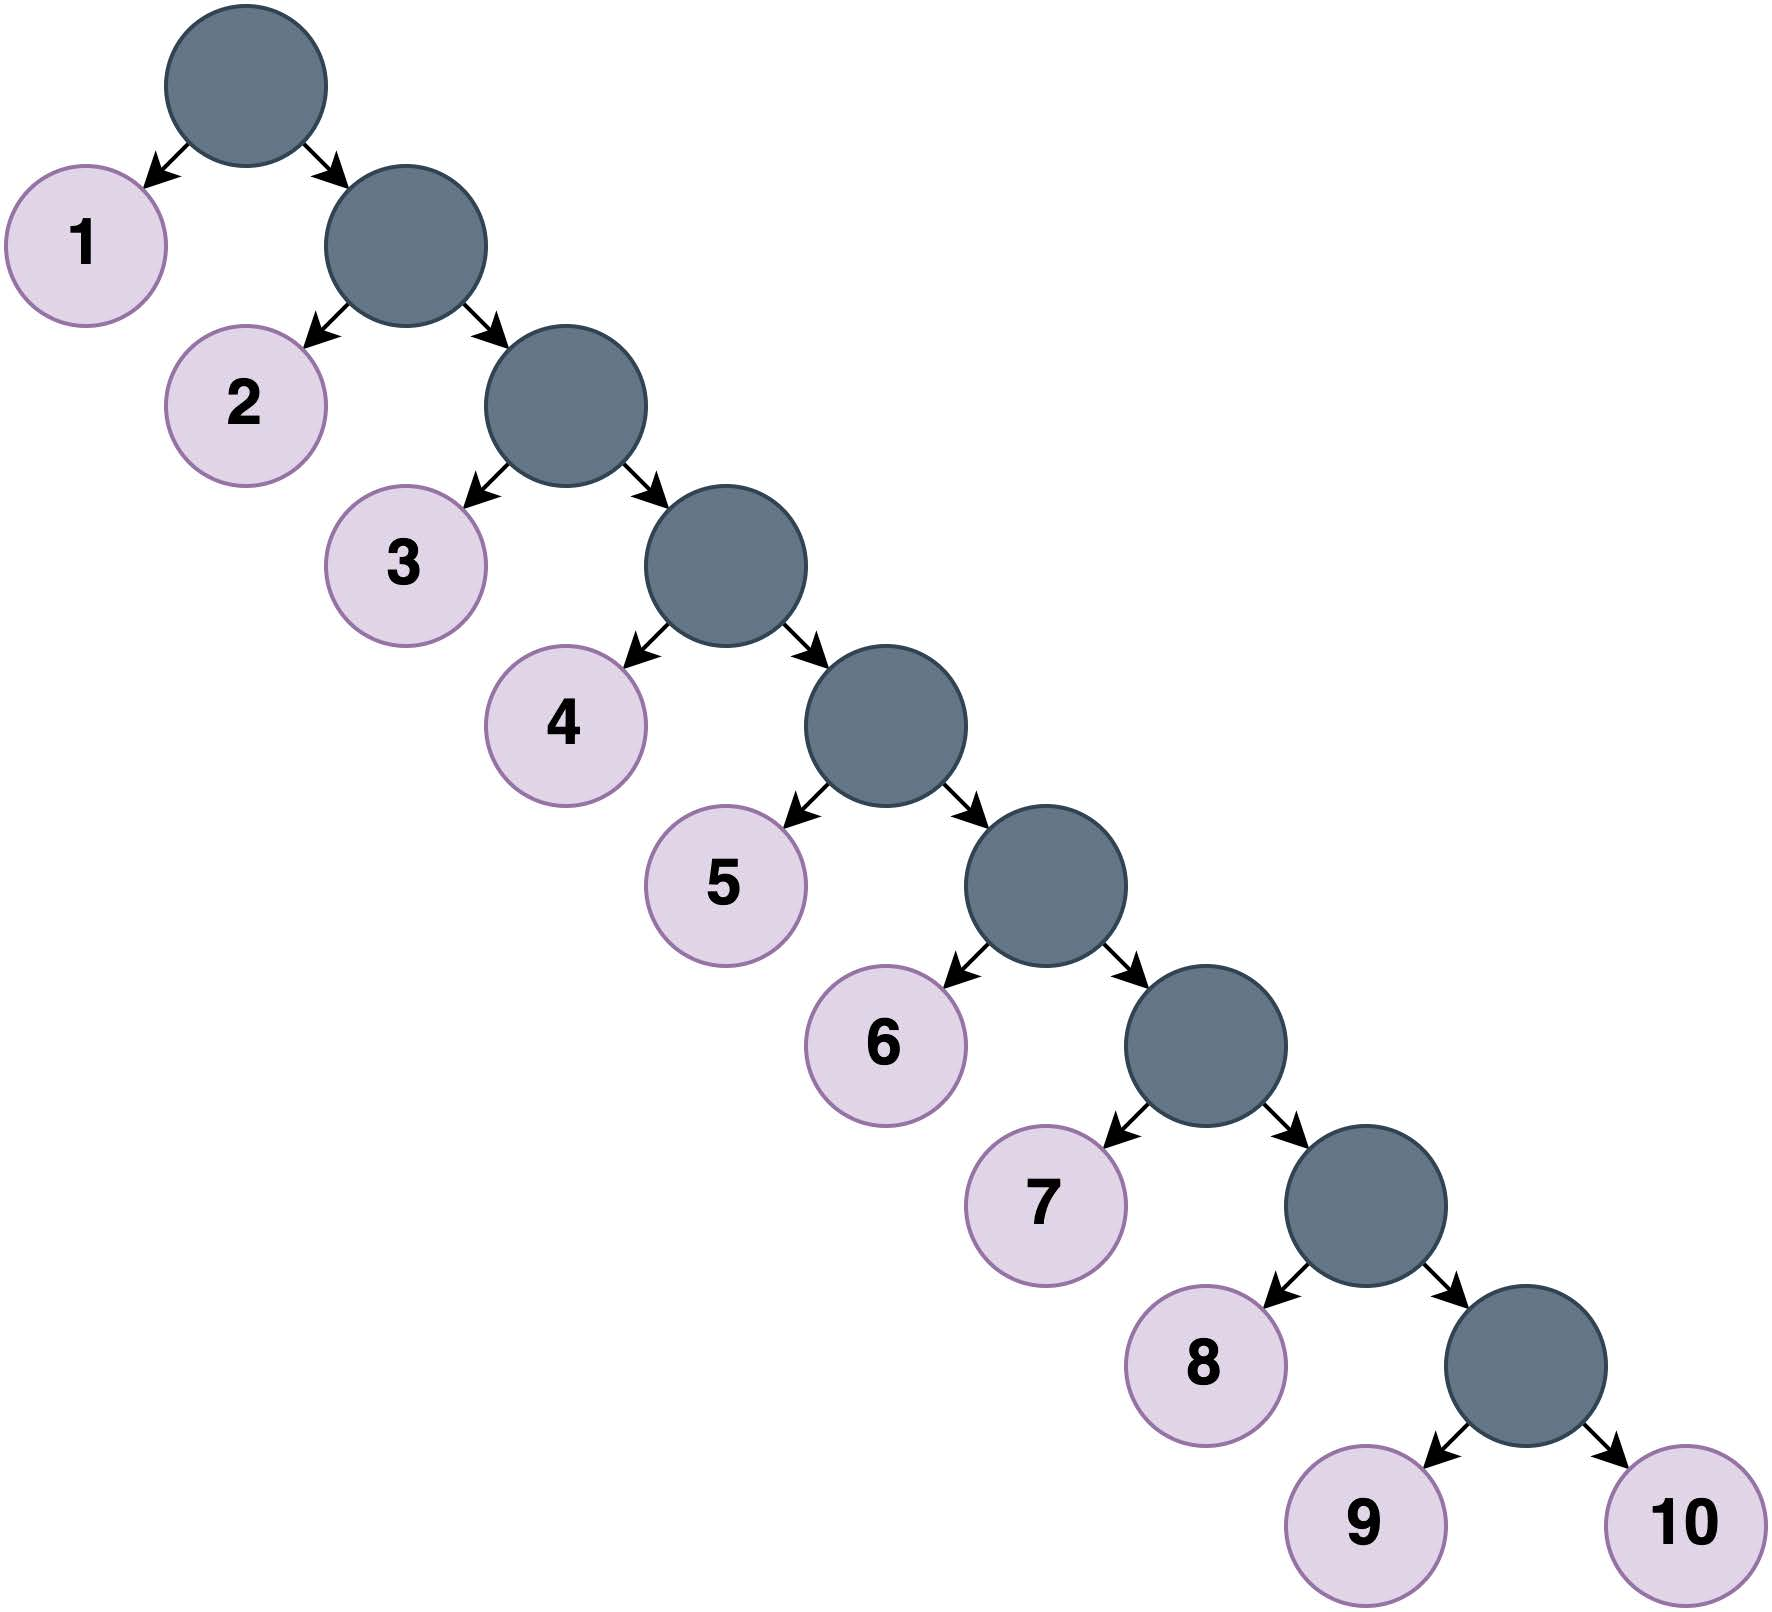
\includegraphics[width=\textwidth]{images/achituve21a.jpg}
                \caption{Multinomial Stick Break Tree}
                \label{fig:imagea1}
            \end{subfigure}
            \hfill
            \begin{subfigure}[b]{0.6\textwidth}
                \centering
                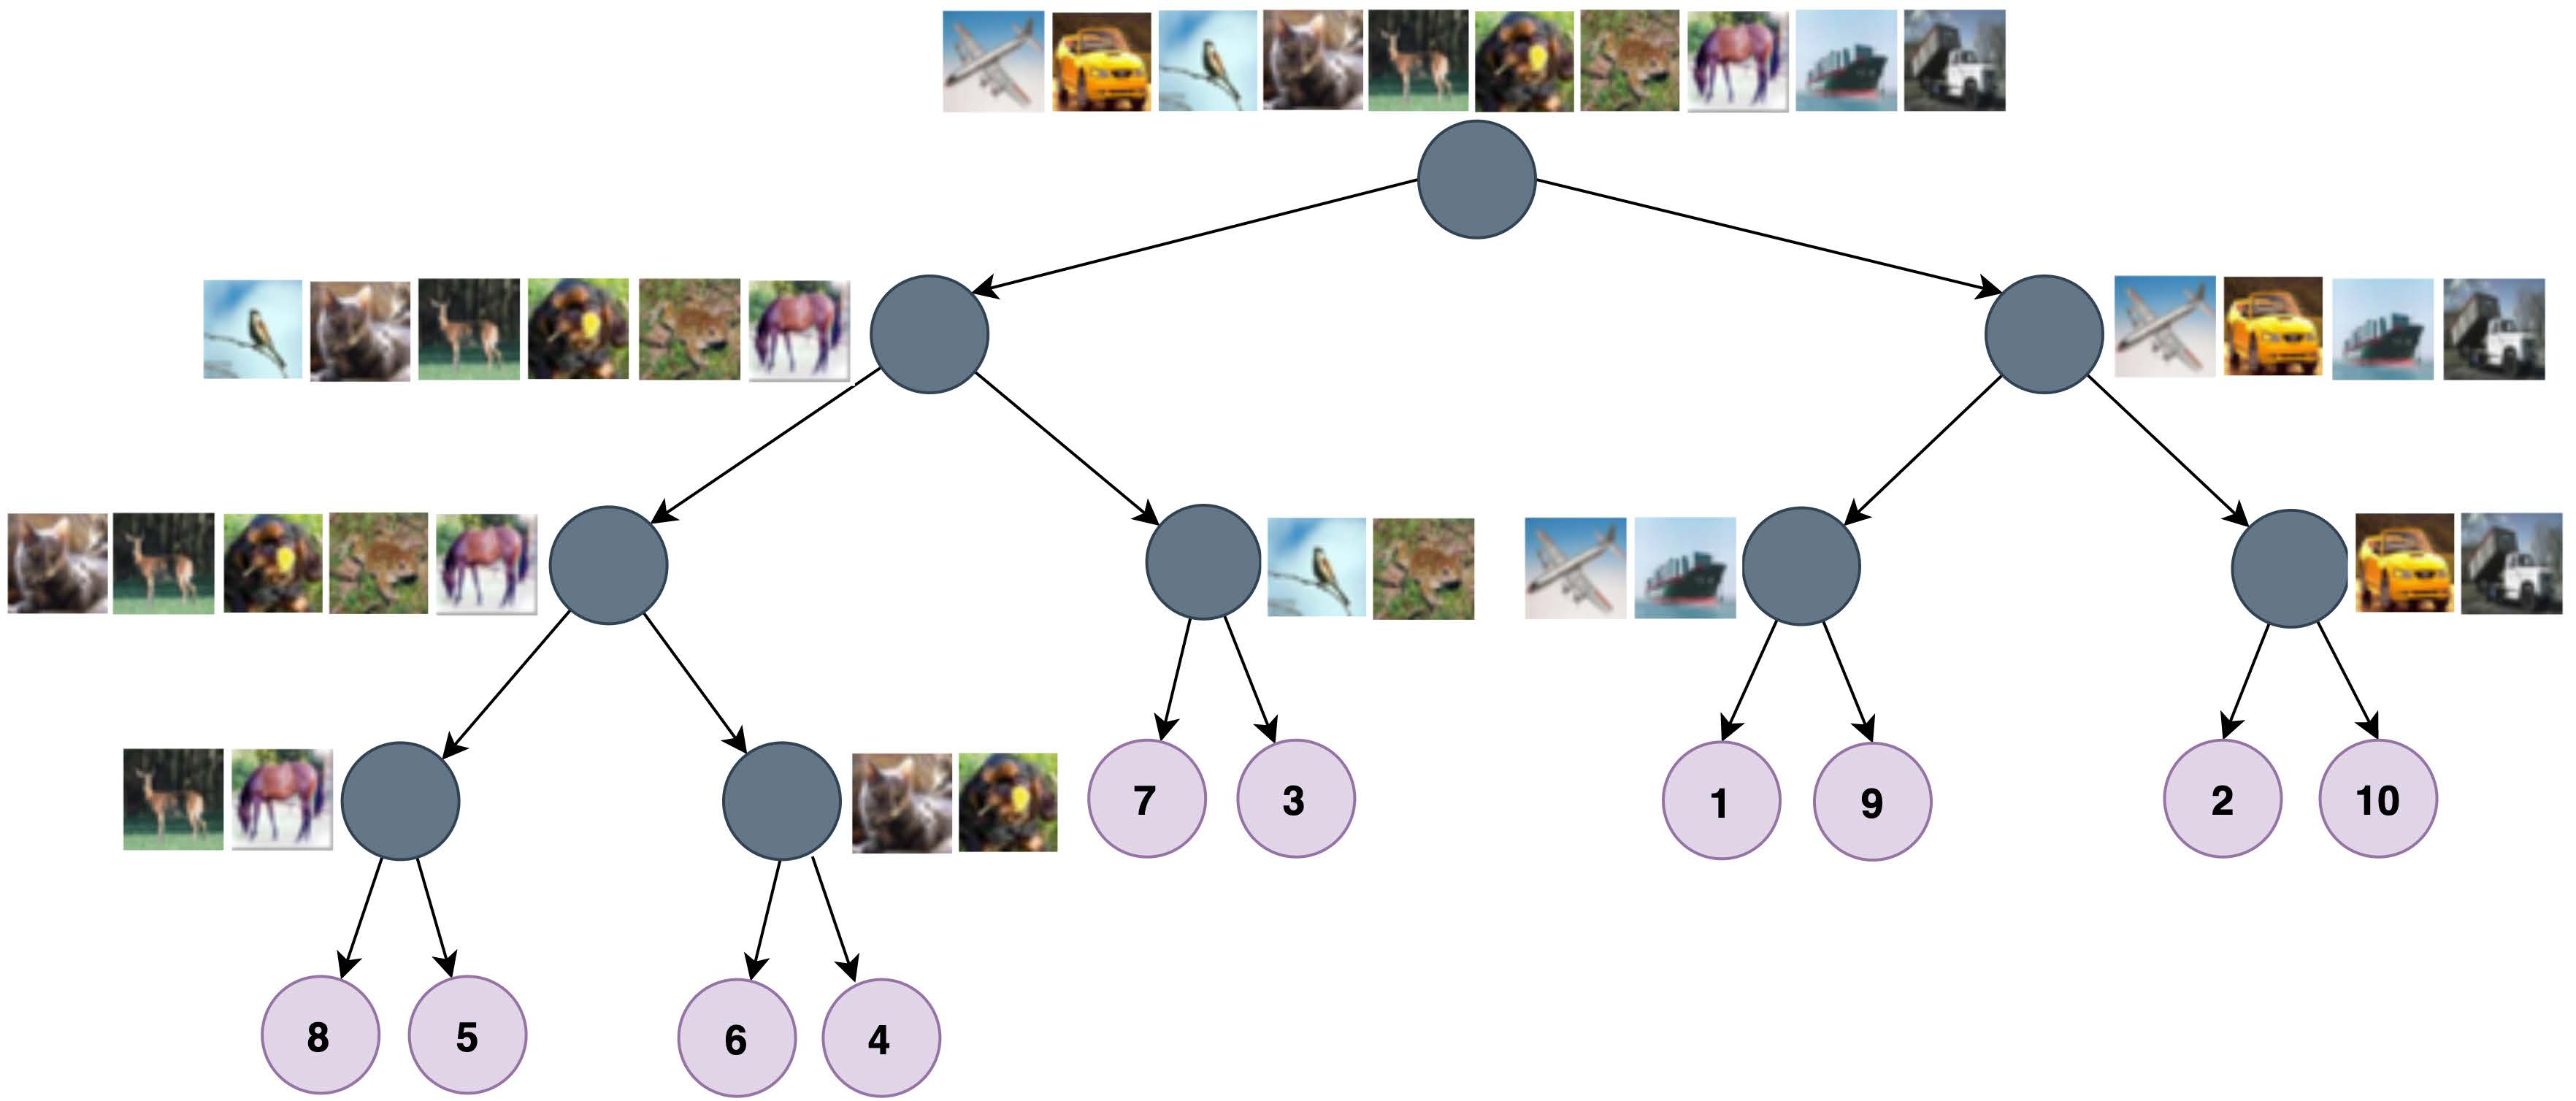
\includegraphics[width=\textwidth]{images/achituve21b.jpg}
                \caption{GP-Tree}
                \label{fig:imageb1}
            \end{subfigure}
            \caption{The trees corresponding to the multinomial stick break model (left) and the GP-Tree model (right) for CIFAR-10. The
            multinomial stick break generates an unbalanced tree in which the order of the classes is arbitrary. GP-Tree, on the other hand, generates a
            more balanced tree that is divided by the semantic meaning of the classes. For example, motorized vehicles are on the right subtree of the
            root node while animals are on the left one. This semantic partition is pronounced at all tree levels.}
            \label{fig:fig1}
        \end{figure}
        \\
        where the remaining probability mass is assigned to the $C_{th}$
        class. While the stick-breaking formulation allows to break
        the multi-class classification problem into a sequence of
        binary classification tasks, as we will show in Section \ref{sec:5.1},        its performance degrades with the number of classes. Intuitively,
        the stick-breaking process can be viewed as a hierarchical
        classification with an extremely unbalanced tree
        (see illustration in Figure \ref{fig:imagea1}. This sequential structure
        can be severely sub-optimal for two reasons: (1) the number
        of binary classification tasks needed to classify a data
        point grows linearly with the number of classes instead of
        logarithmic for a perfectly balanced tree; (2) not all label
        splits result in equally hard binary classification tasks, yet
        the stick-breaking process uses the default label ordering.
        \\
        Therefore, we propose to use a tree-structured hierarchical
        classification instead of the sequential alternative. This
        construction allows finding a tree structure that results in
        easy-to-learn binary tasks. Conceptually, we create a tree
        by splitting the data recursively by classes until we get to
        single class leaves. More formally, starting at the root node,
        we partition the classes $\{1,\ldots,C\}$ into two disjoint sets $C_l$
        and $C_r$, such that $C_l \cup C_r = \{1,\ldots,C\}$. Let $D_l$ and $D_r$
        denote the data points associated with the classes in $C_l$ and
        the classes in $C_r$ respectively. We assign $D_l$ to the left child
        of the root node and $D_r$ to the right one. We recursively
        apply the same operation at each node until we are left with
        single class leaf nodes. Thus, a binary tree is formed (not
        necessarily a perfectly balanced one), see Figure \ref{fig:imageb1} for an
        example. We then fit a binary GP classifier to each internal
        node of the tree that makes a binary decision to either go
        left or go right at that node.
        \\
        The model quality depends on how we partition the data,
        namely the tree construction processes described above. A
        naive approach would be to use a random balanced binary
        tree; however, this strategy does not take advantage of the
        semantic meaning of the classes. We propose the following
        procedure, we first compute a representative prototype for
        each class by taking the mean of all samples (or their representation
        obtained by a NN) belonging to the same class
        coordinate-wise. We then normalize the vectors to have
        unit length and apply divisive hierarchical clustering. We
        recursively split each node by using $k$-means++ clustering
        (\textit{Arthur \& Vassilvitskii, 2007}\cite{arthur2007k}) with $k = 2$ on the class prototype
        vectors, until we are left with single class leaves. We
        note that partitioning the data in this manner may be suboptimal
        when working on the input space directly; however,when applied on features extracted by a NN it is very sensible
        since NNs tend to generate points that cluster around a
        single prototype for each class (\textit{Snell et al., 2017}\cite{snell2017prototypical}). Then, we
        fit a GP to each internal node which makes a binary decision
        based on the data associated with that node. We denote the
        GP associated with node $v_i$ by $f_{v_i}\sim \mathcal{GP}(m_{v_i} , k_{v_i} )$, and all
        of the GPs in the tree with $\mathcal{F}$. The likelihood of a data point
        having the class $c$ is given by the unique path $P^c$ from the
        root to the leaf node corresponding to that class:
        \begin{equation}
            p( y=c|\bm{\mathcal{F}} ) = \prod_{v_i \in P^c}\sigma( f_{v_i})^{y_{v_i}}( 1- \sigma( f_{v_i}))^{ 1 - y_{v_i}} , \label{eq:eq9}
        \end{equation}
        where $y_{v_i} = 1$ if the path goes left at $v_i$ and zero otherwise.
        
        \subsection{Inference at the Node Level}
        \label{sec:3.2}
            Since the likelihood in Eq. \ref{eq:eq9} factorizes over the nodes, we
        may look at the individual components separately. In the
        following we omit the subscript $v_i$ for clarity; however, all
        datum and quantities are those that belong to a specific node
        $v_i$. In general, we can perform inference on each tree node
        with either Gibbs sampling or variational inference (VI).
        For training on large datasets with deep kernel learning and
        inducing points, we found the variational approach to scale
        better, as the inducing points posterior depends on the entire
        dataset. However, when modeling the novel classes in incremental
        few-shot learning, the Gibbs sampling procedure is
        more suitable, as no new parameters are required.
        \\
        For Gibbs sampling, we use the posterior probabilities introduced
        in section \ref{sec:2.3}. At each node, we can use block-Gibbs
        sampling to sample $\bm{\omega}$ and $\bm{f}$. Then we can obtain the augmented
        marginal and predictive distributions described next.
        The augmented marginal likelihood:
        \begin{equation}
            \label{eq:eq10}
            p( \bm{y}|\bm{\omega},\bm{X} ) = \int p( \bm{y}|\bm{f},\bm{\omega},\bm{X} )p(\bm{f})d\bm{f} \propto \mathcal{N} ( \bm{\Omega}^{-1} \bm{\kappa} | \textbf{0}, \bm{K}+\bm{\Omega}^{-1}),
        \end{equation}
        and the augmented predictive likelihood on a new data point
        $x_*$:
        \begin{equation}
        \label{eq:eq11}
            p( y_*|\bm{x}_*,\bm{\omega},\bm{y},\bm{X}  ) = \int p( y_*|f_*)p( f_*|\bm{x}_*,\bm{\omega}_*,\bm{y},\bm{X} )df_*,
        \end{equation}
        where,
        \begin{align}
        \label{eq:eq12}
            p( f_*|\bm{x}_*,\bm{X},\bm{y},\bm{\omega}  ) &= \mathcal{N}( f_*|\mu_*,\Sigma_* ),\nonumber \\
            \mu_* &= \bm{k}_*^T( \bm{\Omega}^{-1}+\bm{K} )^{-1}\bm{\Omega}^{-1}\bm{\kappa},\\
            \Sigma_* &= k_{**} - \bm{k}_*^T( \bm{\Omega}^{-1}+\bm{K} )^{-1} \bm{k}_{**}.\nonumber
        \end{align}
                Where we assumed a zero mean prior. The integral in Eq. \ref{eq:eq11}
        is intractable but can be computed numerically with 1D
        Gaussian-Hermite quadrature.
        \\
        Alternatively to the Gibbs sampling, we may apply variational
        inference at each node. We define $\bm{\Bar{X}}$
        as the learned
        pseudo-inputs and $ \bm{\Bar{y}}$ as their associated class labels. $\bm{\Bar{X}}$
        are defined at the tree level and are shared by all relevant
        nodes. For each node we define the variational distributions
       $ q(\bm{\omega}) = PG(1, \bm{c})$ and $q( \bm{\Bar{f}}) = \mathcal{N}( \bm{\Bar{f}}|\Tilde{\bm{\mu}}, \Tilde{\bm{\Sigma}})$, where c, $\Tilde{\bm{\mu}}$,$\Tilde{\bm{\Sigma}}$
        are learnable parameters. The variational lower bound to
        the log marginal likelihood is:
        \begin{equation}
        \label{eq:eq13}
            \mathcal{C}(\bm{c},\bm{\Tilde{\bm{\mu}}},\bm{\Tilde{\bm{\Sigma}}}) = \mathbb{E}_{p( \bm{f} | \bm{\Bar{f}} ) q(\bm{\Bar{f}})q(\bm{\omega}) } [ \log \,p( \bm{y}|\bm{\omega}, \bm{f}) - KL( q( \bm{\Bar{f}},\bm{\omega} )|| p( \bm{\Bar{f}},\bm{\omega} ) ) ]
        \end{equation}
        which has a closed-form expression. We can then learn
        the model parameters and the variational parameters by maximizing the variational lower bound in Eq. \ref{eq:eq13}. The
        explicit form of Eq. \ref{eq:eq13} and the update rules of the variational
        parameters were adapted from (\textit{Wenzel et al., 2019}\cite{wenzel2019efficient}) and are
        presented in supplementary Section A.
        \\
        To make predictions we can plug in the approximate posterior
        in the predictive posterior calculation:
        \begin{equation}
        \label{eq:eq14}
        \begin{aligned}
            p( f_*|x_*,\bm{\Bar{X}},\bm{\Bar{y}} ) &\approx \int p( f_*|\bm{\Bar{f}},x_* )q( \bm{\Bar{f}} )d\bm{\Bar{f}} \\
            &= \mathcal{N}( f_*|\mu_*,\Sigma_* ), \\
            \mu_* &= \bm{k}_{m*}^T\bm{K}_{mm}^{-1}\Tilde{\bm{\mu}}, \\
            \Sigma_* &= k_{**}-\bm{k}_{m*}^T( \Tilde{\bm{\Sigma}}\bm{K}_{mm}^{-1} - I )k_{m*},
        \end{aligned}
        \end{equation}
        where $\bm{k}_{m*}$ denotes the kernel vector between the inducing
        points and the test point, and $k_{**}$ denotes the kernel value
        at the test point. Similarly to the Gibbs sampling case,
        we can obtain $p( y_*|x_*,\bm{\Bar{y}},\bm{\Bar{X}} )$ by taking an integral over
        $f_*$ and compute it numerically with 1D Gaussian-Hermite
        quadrature.
        \subsection{Full Learning of the Tree}
        \label{sec:3.3}
        We discussed how to learn and perform inference on a single
        node, we will now describe how to train the full tree model.
        For the full tree we need to learn the joint pseudo-inputs and
        the per-node variational parameters. Optimizing the full tree
        splits into the separate marginal likelihood of all examples
        and all the nodes on the path from the root to the leaf nodes:
        \begin{equation}
        \label{eq:eq15}
            \begin{aligned}
            \mathcal{L} &= \sum_{j=1}^n \log p( y_i|\bm{x_j},\bm{\Bar{y}},\bm{\Bar{X}} )\\
            &= \sum_{j=1}^n \sum_{v_i \in P^{y_j}} \log p( y_{v_i}|\bm{x_j},\bm{\Bar{y}},\bm{\Bar{X}} )
            \end{aligned}
        \end{equation}
        Since we cannot directly optimize this loss, we optimize
    the lower bound of it given in Eq. \ref{eq:eq13}. We summarize the
    learning algorithm of GP-Tree with VI in supplementary
    Section B. To apply predictions in the original multi-class
    problem, the prediction for a new data point $x_*$ is given as
    the product of predictive distributions from the root node to
    leaf node corresponding to each class.
    \\
    Our method can be easily integrated with DKL. We simply
    superimpose the tree-based GP on an embedding layer of a
    neural network and learn the network parameters $\theta$ as well.
    In this case, we may define the inducing inputs in the input
    space or the feature space. We found that setting them in
    the feature space yields better performance, and requires
    less memory. Their location was initialized at the beginning
    of training using k-means++ applied on the embedding of
    data samples for each class separately. Also, we empirically
    found it beneficial to start the training process with a few
    epochs of standard training using the cross-entropy loss before building the GP tree and transitioning to learning
    with it.
        \begin{figure}
            \centering
            \begin{subfigure}[b]{0.25\textwidth}
                \centering
                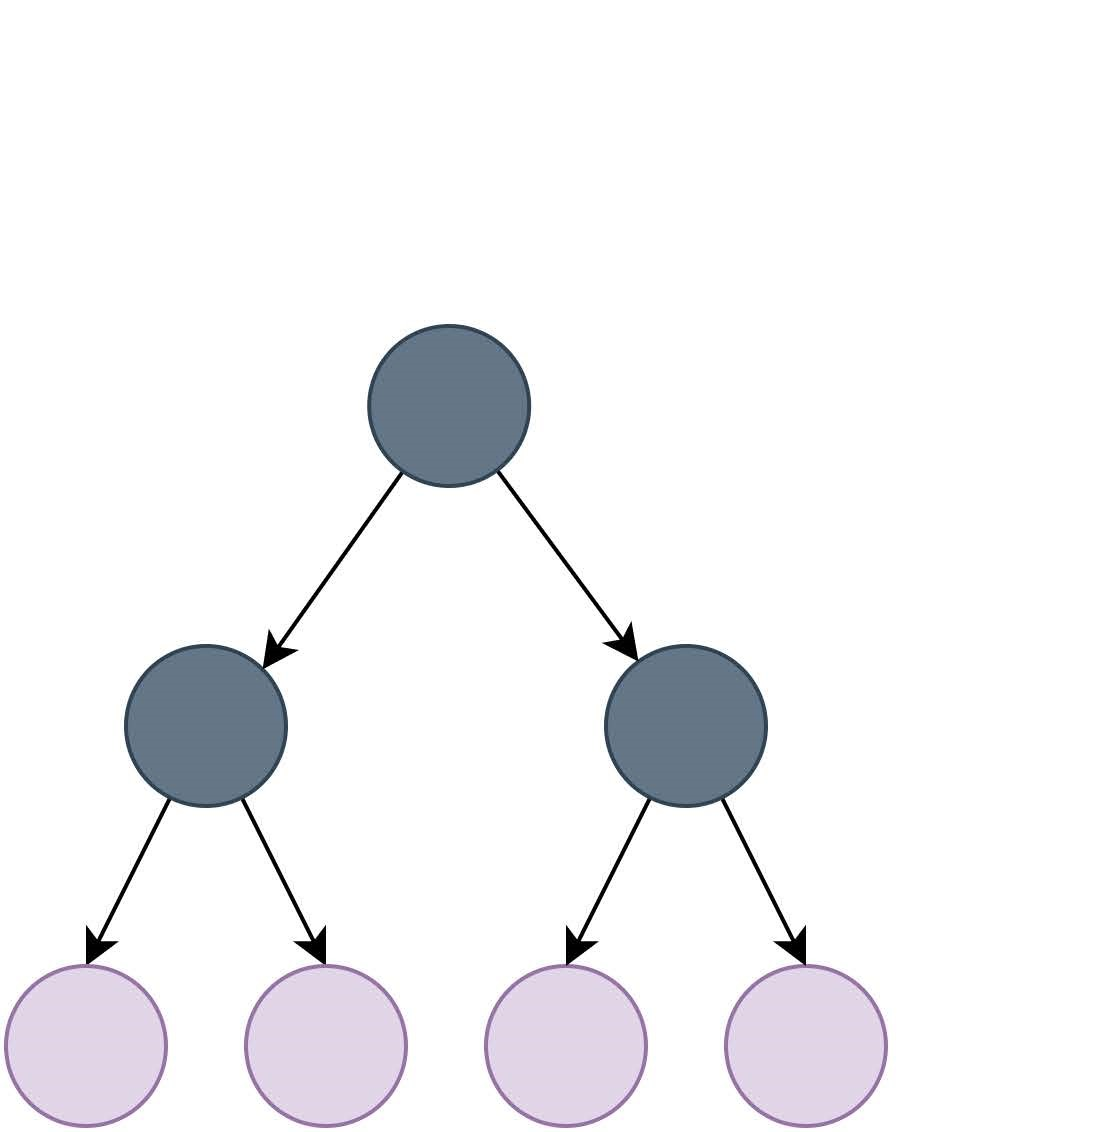
\includegraphics[width=\textwidth]{images/achituve21c1.jpg}
                \caption{Base}
                \label{fig:imagea2}
            \end{subfigure}
            \hfill
            \begin{subfigure}[b]{0.25\textwidth}
                \centering
                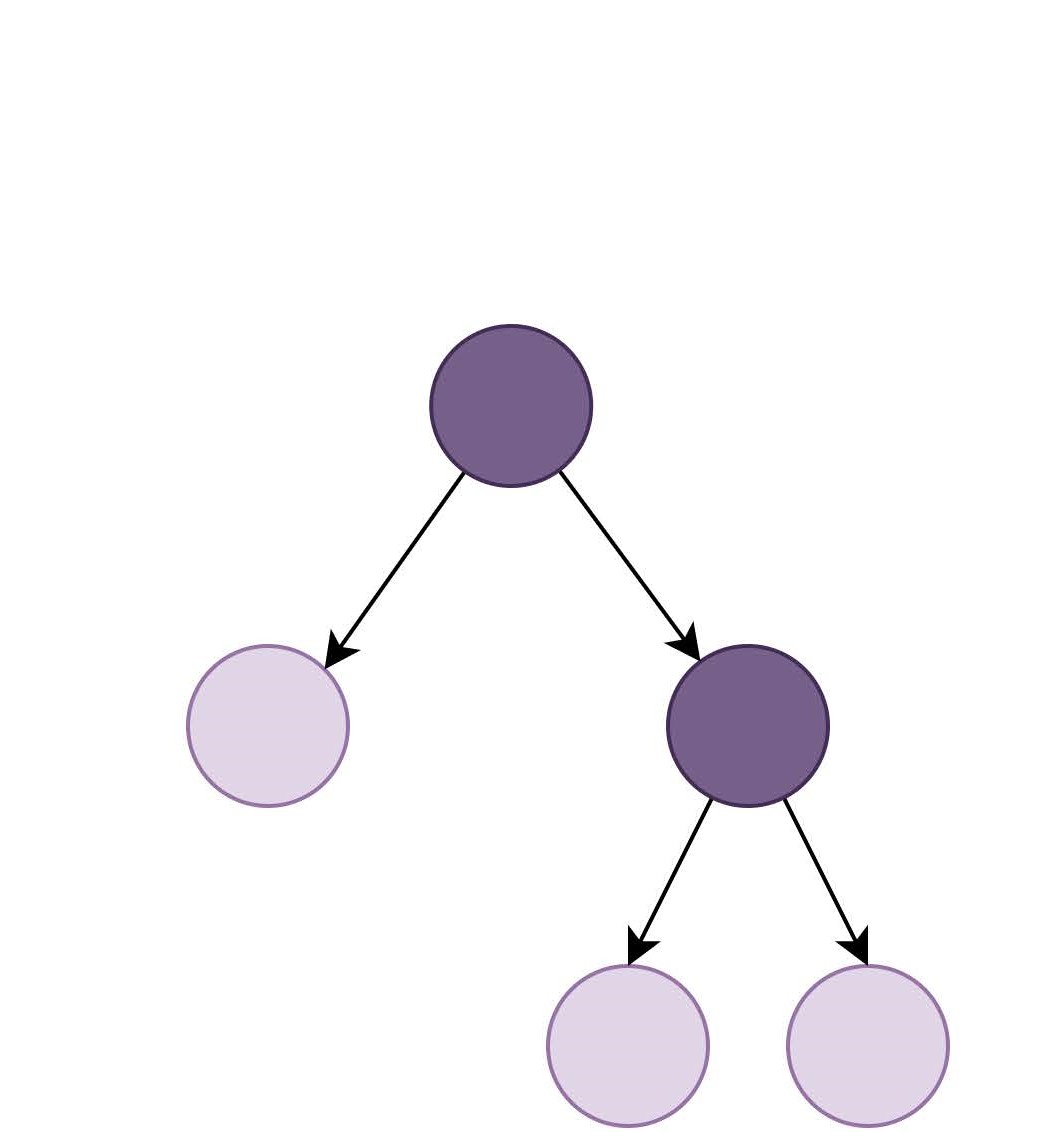
\includegraphics[width=\textwidth]{images/achituve21c2.jpg}
                \caption{Novel}
                \label{fig:imageb2}
            \end{subfigure}
            \hfill
            \begin{subfigure}[b]{0.4\textwidth}
                \centering
                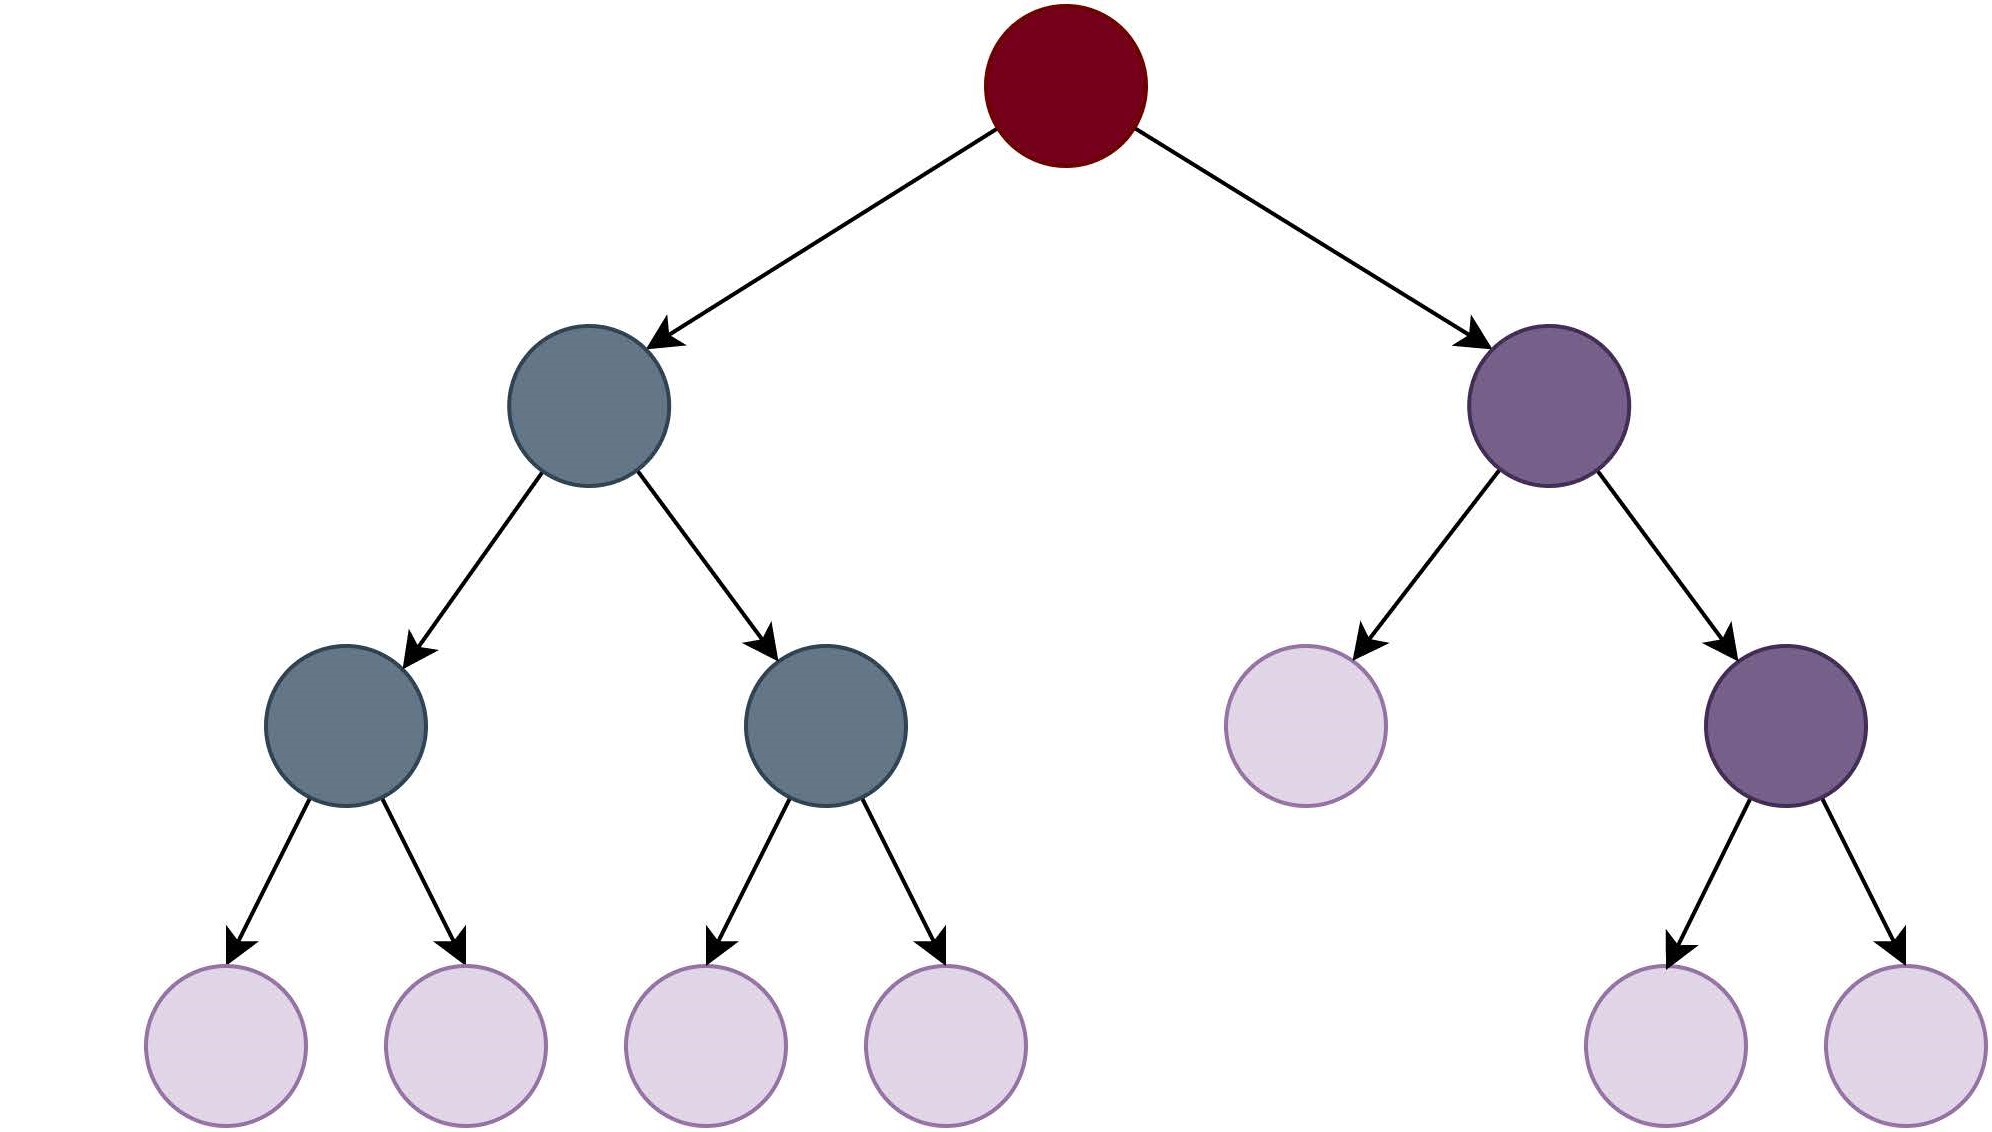
\includegraphics[width=\textwidth]{images/achituve21c3.jpg}
                \caption{Shared}
                \label{fig:imagec2}
            \end{subfigure}
            \caption{Tree expansion for novel classes: (a) A tree that was
            learned on the base classes; (b) On a novel session, we first build a
            tree from the novel classes representations; (c) Next we connect
            the trees using a shared root node.}
            \label{fig:fig2}
        \end{figure}

    \subsection{GP-Tree for Few-Shot Class-Incremental Learning}
    \label{sec:3.4}
        In class-incremental learning, we are given a sequence of
        labeled datasets $D_1,D_2,\ldots,D_T$ , each sampled from a disjoint
        set of classes $C_1,\ldots,C_T$ . At each timestamp $t$, the
        model has access to dataset $D_t$ and the previous model, and
        it is tasked with classifying all the previously seen classes
        $\cup_{i=1}^t
        C_i$. In few-shot incremental learning (\textit{Ren et al., 2019}\cite{ren2019incremental};
        \textit{Tao et al., 2020}\cite{tao2020few}), the base classes dataset, $D_1$, have a large
        number of samples, but all of the following datasets ($D_2$ onwards)
        have a limited amount of labeled data, e.g., 5 samples
        per class. Thus, after the model learned the previous classes
        it is tasked with learning new classes from few examples
        and without impairing the classification of previously seen
        classes whose data isn’t available at that time, also known as
        catastrophic forgetting (\textit{McCloskey \& Cohen, 1989}\cite{mccloskey1989catastrophic}). Gaussian
        processes are naturally well-suited for this challenge.
        Bayesian models generalize well from few examples (\textit{Snell
        \& Zemel, 2021}\cite{snell2021bayesian}) and the inducing points can be used as
        a compact representation of the base classes, allowing us
        to avoid catastrophic forgetting. As Gaussian processes
        are non-parametric learners, we can classify new classes
        without fitting any new variables or tuning the NN parameters,
        which may also mitigate the catastrophic forgetting
        problem.
        \\
        \\
        At the initial phase of learning the base classes, we employ
        GP-Tree (with DKL) to learn this dataset using VI as described
        earlier. We can view the inducing inputs, which
        are learned per class, as ’exemplars’ of the base classes, a
        commonly used practice in incremental learning studies (\textit{He
        et al., 2018}\cite{he2018exemplar}). We then use them in future learning sessions
        as described next. At the end of this stage, we freeze the
        NN backbone to avoid any parameter learning.
        \\
        \\
        At each new session, we are given data from novel classes.
        We use the (fixed) NN backbone to obtain representations
        for the new samples that will be used for modeling the novel
        classes with GP-Tree. In this case, unlike the learning of
        base classes, the datasets are small. Therefore, we do not need to use inducing points. We just need to restructure the
        tree to account for the new classes and fit a GP to each new
        node. There are several alternatives for restructuring the
        tree, here we propose the following. We retain the original
        tree that was learned on the base classes intact, and at each
        novel session, we build a sub-tree from the embedding of
        samples in all (novel) sessions until the current one, namely
        $D_2, \ldots,D_t$. We refer to these examples as novel examples
        hereafter. We then connect the sub-tree of novel examples
        with the sub-tree of the base classes with a shared root node.
        We define a GP classifier for each node in the sub-tree of
        novel examples and the root node. The GPs for the nodes in
        the sub-tree of the base classes are left untouched. Fitting
        the GPs in the sub-tree of novel examples is easily done
        with the representation of all examples at hand. For the root
        node, since we no longer have the base classes examples,
        we may use the inducing inputs of the base classes along
        with the embeddings of the novel examples. See illustration
        in Figure \ref{fig:fig2}. We use Gibbs sampling on all new nodes to
        avoid any parameter tuning after the initial training on the
        base classes. Supplementary Section D.2 presents other
        alternatives for constructing the tree at novel sessions.
        \\
        \\
        It is important to note that while we do save the inducing
        inputs and the network representations of samples from
        novel sessions for future sessions, this is in line with other
        incremental learning studies that save a few samples per
        class (\textit{Douillard et al., 2020}\cite{douillard2020podnet}). Furthermore, we only save
        the embeddings and not the original images. Therefore,
        the memory costs are low and in practice are negligible
        compared to storing the trained network weights. Also,
        we emphasize that the method described here is a natural
        way to extend our classification model to new classes. It
        was not tailored for the class-incremental few-shot scenario
        specifically. Despite that, we show strong results compared
        to models designed specifically for this task, especially on
        later learning sessions (see Section \ref{sec:5.3}). Finally, GP-Tree
        can be easily extended to standard incremental learning
        setups. One immediate option is to build a tree and learn
        inducing inputs only for the novel classes seen at each new
        session similarly to the learning applied for base classes
        with VI. Then this sub-tree can be connected to the previous
        tree with a shared root node. This strategy can be further
        improved by taking only the inducing inputs from all classes
        seen thus far at the end of each novel session to rebuild the
        entire tree. Then we can use either the VI approach or,
        preferably, our Gibbs sampling procedure. In this study, we
        focus on the few-shot case and we leave this extension to
        future work.

    \section{Related Work}
    \label{sec:4}
    \textbf{Incremental learning.} Incremental learning (IL) aims at
    learning new data without forgetting old data, what is known as ’catastrophic forgetting’ (\textit{McCloskey \& Cohen, 1989}\cite{mccloskey1989catastrophic}).
    Recently, a large body of research was done in that direction,
    most of which is based on methods that use NNs only. Notable
    studies that use a similar procedure to ours are \textit{Titsias
    et al. (2019)}\cite{titsias2019functional} which regularize subsequent tasks with a set
    of inducing points stored from previous tasks, and \textit{Gidaris
    \& Komodakis (2018)}\cite{gidaris2018dynamic} which also freeze the feature extractor
    after learning the base classes and infer a classification
    weight vector for novel categories. Methods in this field
    can be categorized according to three types: (i) \textit{Regularization
    based} approaches impose regularization methods on
    the network to maintain past knowledge (\textit{Goodfellow et al.,
    2014}\cite{goodfellow2014catastrophic}; \textit{Kirkpatrick et al., 2017}\cite{kirkpatrick2017overcoming}; \textit{Lee et al., 2017}\cite{lee2017overcoming}; \textit{Chaudhry
    et al., 2018}\cite{chaudhry2018riemannian}; \textit{Schwarz et al., 2018}\cite{schwarz2018progress}; \textit{Ren et al., 2019}\cite{ren2019incremental}). For
    example, \textit{Kirkpatrick et al. (2017)}\cite{kirkpatrick2017overcoming} limit the update of the
    parameters when encountering new data based on the fisher
    matrix ; (ii) \textit{Architectural based} methods suggest network
    architectures that are resilient to the catastrophic forgetting
    issue and can accommodate new tasks (\textit{Mallya et al., 2018}\cite{mallya2018packnet};
    \textit{Mallya \& Lazebnik, 2018}\cite{mallya2018piggyback}; \textit{Yoon et al., 2018}\cite{yoon2018lifelong}; \textit{Serra et al.,
    2018}\cite{serra2018overcoming}; \textit{Taitelbaum et al., 2019}\cite{taitelbaum2019network}; \textit{jun Liu et al., 2020}\cite{liu2020mnemonics}). For example,
    \textit{Rusu et al. (2016)}\cite{rusu2016progressive} and following it \textit{Yoon et al. (2018)}\cite{yoon2018lifelong}
    expend the network with each new task. When applying
    parameters update the former freezes the previous network
    while the latter retrain part of it; (iii) \textit{Rehearsal based} aims
    at preventing catastrophic forgetting by storing and replaying
    information from previous episodes (\textit{Rebuffi et al., 2017}\cite{rebuffi2017icarl};
    \textit{Castro et al., 2018}\cite{castro2018end}; \textit{Wu et al., 2018}\cite{wu2018memory}; \textit{Hou et al., 2019}\cite{hou2019learning}; \textit{Zhai
    et al., 2019}\cite{zhai2019lifelong}; \textit{Liu et al., 2020b}\cite{liu2020when}; \textit{jun Liu et al., 2020}\cite{liu2020more}). \textit{Rebuffi
    et al. (2017)}\cite{rebuffi2017icarl} introduced the class-incremental learning setup.
    They used exemplars to maintain information of past data
    and applied the nearest-mean-of-exemplars classification
    rule. In this paper, we follow the protocol suggested by (\textit{Tao
    et al., 2020}\cite{tao2020few}) for few-shot class-incremental learning.
    \\
    \\
    \textbf{Gaussian process classification.} In GPs for classification
    tasks the likelihood is no longer Gaussian and therefore
    approximation-based approaches or Monte-Carlo-based approaches
    are needed. Some classic non-augmentation based
    methods include the Laplace approximation (\textit{Williams \&
    Barber, 1998}\cite{williams1998bayesian}), expectation-propagation (\textit{Minka, 2001}\cite{minka2001family}), and
    the least square approach (\textit{Rifkin \& Klautau, 2004}\cite{rifkin2004defense}). We
    refer the readers to (\textit{Rasmussen \& Williams, 2006}\cite{rasmussen2006gaussian}) for a
    more thorough review. Recently some approaches emerged
    that are based on the Pólya-Gamma augmentation (\textit{Polson
    et al., 2013}\cite{polson2013bayesian}). \textit{Linderman et al. (2015)}\cite{linderman2015dependent} proposed to use the
    Pólya-Gamma in a stick-breaking process to reparameterize
    a multinomial distribution as a product of binomial distributions.
    \textit{Wenzel et al. (2019)}\cite{wenzel2019efficient} proposed to use Pólya-Gamma
    augmentation with variational inference for binary classification
    tasks. \textit{Galy-Fajou et al. (2020)}\cite{galy2020multiclass} proposed to use the
    logistic softmax likelihood and derived a conditionally conjugate
    model based on three augmentation steps. We believe
    that the quality of the prediction and learning may degrade as a result of the cascade of approximations. \textit{Snell \& Zemel
    (2021)}\cite{snell2021bayesian} proposed to use the one-vs-each likelihood in a few
    shot setting. Their method does not scale well with the data
    and classes due to the inversion of a $CN \times CN$ matrix. We
    use a Gibbs sampling approach for learning novel classes
    at each node. Several studies suggested alternative, more
    efficient, posterior sampling techniques when the classes are
    imbalanced or when using sub-samples of the data (\textit{Nemeth
    \& Fearnhead, 2020}\cite{nemeth2020stochastic}; \textit{Sachs et al., 2020}\cite{sachs2020posterior}; \textit{Sen et al., 2020}\cite{sen2020efficient}). Using
    such techniques to improve the standard Gibbs sampler
    is out of the current study scope.
    \\
    \\
    \textbf{Scalable GPs.} In recent years some attempts were made
    to make GP classification more scalable. Inducing points
    (\textit{Silverman, 1985}\cite{silverman1985some}; \textit{Quinonero-Candela \& Rasmussen, 2005}\cite{quinonero2005unifying};
    \textit{Snelson \& Ghahramani, 2006}\cite{snelson2006sparse}) are a popular method to
    handle large datasets. \textit{Hoffman et al. (2013)}\cite{hoffman2013stochastic} developed
    a stochastic optimization process for VI. \textit{Hensman et al.
    (2015)}\cite{hensman2015scalable} introduced a method for GPC within a variational inducing
    point framework. \textit{Izmailov et al. (2018)}\cite{izmailov2018scalable} used tensor
    train decomposition for variational parameters that allowed
    increasing dramatically the number of inducing points. \textit{Wilson
    et al. (2016b)}\cite{wilson2016stochastic} proposed to learn multiple GPs on an embedding
    space and combine them linearly before a Softmax
    function. Extending this method to the incremental learning
    setting is not immediate as there are learnable parameters
    for combining the classes. \textit{Bradshaw et al. (2017)}\cite{bradshaw2017adversarial} used a
    GP with the Robust-Max likelihood for robustness against
    adversarial examples. This method doesn’t scale well with
    the number of classes as we will show in Section \ref{sec:5.2}.
    \\
    \\
    \textbf{Hierarchical models.} Hierarchical classifiers are a popular
    design choice. \textit{Morin \& Bengio (2005)}\cite{morin2005hierarchical}, and following
    it \textit{Mnih \& Hinton (2008)}\cite{mnih2008scalable} proposed a tree-based classifier
    for language modeling. Their method applies to situations
    where all words are known in advance, while we need the
    ability to dynamically adapt the tree with new classes. \textit{Damianou
    \& Lawrence (2013)}\cite{damianou2013deep} stacked multiple GPs to create a
    hierarchy of GPs. \textit{Nguyen et al. (2019)}\cite{nguyen2019scalable} proposed a hierarchical
    model using a mixture of GPs to learn global and
    local information. However, it is not clear how to extend
    this method to incremental learning challenges.
    Hierarchical stick break process was used in several contexts
    as well. \textit{Adams et al. (2010)}\cite{adams2010treestructured} proposed a tree-based
    stick break for clustering as an alternative to the standard
    sequential stick break. \textit{Nassar et al. (2019)}\cite{nassar2019tree} proposed to use
    a tree-structure stick break for linear dynamical systems.
    Both methods did not include any GP components and do
    not have the flexibility of our model to apply inference with
    either VI or Gibbs sampling.
    \begin{table}
    \centering
    \caption{Test accuracy on CUB-200-2011. Average over 10 runs $\pm$( SEM). In bold: statistically significant best results (p=0.05).}
    \label{tab:table1}
    \resizebox{\textwidth}{!}{
    \begin{tabular}{lccccccccc}
    \Xhline{2\arrayrulewidth}
    \multirow{2}{*}{Method} & \multicolumn{9}{c}{Number of Classes}     \\
    \cline{2-10}
                      &4& 6 & 8 & 10 & 20 & 30 & 40 & 50 & 60  \\
                      \hline
                      SBM-GP  & 96.98$\pm$0.5 & 95.55$\pm$0.9 & 92.11$\pm$0.8 & 91.04$\pm$0.7 & 83.59$\pm$0.5 & 77.63$\pm$0.9 & 67.03$\pm$0.8 &64.20$\pm$1.0 & 60.69$\pm$1.0\\
                      OVE & 97.33$\pm$0.5 & 96.60$\pm$0.9 & 94.70$\pm$0.8 & 93.05$\pm$0.8 & - & - & - & - &-\\
                      LSM & 97.30$\pm$0.9 & 96.95$\pm$0.8 & 95.16$\pm$0.8 & 93.09$\pm$0.9 & 89.23$\pm$1.3 & 84.44$\pm$0.6 & 72.90$\pm$1.2 & 69.82$\pm$0.9 & 65.53$\pm$0.9\\
                      \hline
                      GP-Tree Rnd. (ours) & 97.80$\pm$0.8 & 95.96$\pm$0.7 & 93.49$\pm$0.9&92.07$\pm$1.1 & 85.32$\pm$1.6 & 77.45$\pm$1.0 & 68.97$\pm$0.8 & 62.77$\pm$1.2 & 58.49$\pm$0.8 \\
                      GP-Tree (ours) &  97.93$\pm$0.7& 97.15$\pm$0.6 & 94.67$\pm$0.9 & 93.57$\pm$0.9 & 88.77$\pm$1.4&83.87$\pm$0.8 & \textbf{75.66$\pm$0.8} & \textbf{72.87$\pm$0.8} & \textbf{69.92$\pm$0.6}\\
                      \Xhline{2\arrayrulewidth}
    \end{tabular}}
    \end{table}
    
    \section{Experiments}
    \label{sec:5}
    In our experiments, we first examine several aspects of our
    method compared to previous common GPC methods (Sections
    \ref{sec:5.1} \& \ref{sec:5.2}). Then we evaluate GP-Tree on the setting of
    class incremental few-shot learning (Section \ref{sec:5.3}). In the supplementary
    material we provide full implementation details
    (Section C), ablation study, and further analysis (Section D).
        \subsection{Inference With Gibbs Sampling}
        \label{sec:5.1}
        As described in Section \ref{sec:3}, GP-Tree allows to do inference
        with Gibbs sampling. This method is preferable when modeling
        novel classes in incremental learning, as we do not
        want to optimize any parameters and the size of the datasets
        are small. We evaluated GP-Tree in this setup on the finegrained
        classification dataset, Caltech-UCSD Birds (CUB)
        200-2011 (\textit{Welinder et al., 2010}\cite{welinder2010caltech}). The CUB dataset contains
        11,788 images of bird species from 200 classes with approximately
        30 examples per class in the training set. Here,
        we did not apply DKL, but rather we used the pre-trained
        features published by (\textit{Xian et al., 2018}\cite{xian2018feature}). This allowed us to
        only compare the inference part of our model.
        \\
        \\
        We compared GP-Tree against the following baselines that
        also used the Pólya-Gamma augmentation to get a conditionally
        conjugate likelihood: \textbf{(1) Stick Break Multinomial
        GP (SBM-GP)} (\textit{Linderman et al., 2015}\cite{linderman2015dependent}): that used the
        stick-breaking process to convert a multinomial likelihood
        to a product of binomial likelihoods; \textbf{(2) Logistic-Softmax
        (LSM)} (\textit{Galy-Fajou et al., 2020}\cite{galy2020multiclass}) a recent method for GPC
        based on the logistic-softmax likelihood; and \textbf{(3) One-vs-Each (OVE)} (\textit{Snell \& Zemel, 2021}\cite{snell2021bayesian}) a method for GPC proposed
        recently for few-shot learning. Because this method
        requires the inversion of a $CN \times CN$ matrix, we were able to run it with only a few classes.
        \\
        \\
        Table \ref{tab:table1} compares GP-Tree against the baseline methods
        at increasing number of classes starting from 4 to 60 (out
        of 200). The results are the average test-set classification
        accuracy along with the standard error of the mean (SEM)
        over ten seeds which included randomization in the class
        selection. When the number of classes is small ($\leq$ 30)
        GP-Tree, LSM, and OVE are comparable. However, as
        the number of classes increases GP-Tree performs better.
        Table 1 also shows a variant of GP-Tree in which a balanced
        tree is built based on a random split of the classes (\textbf{GP-Tree
        Rnd}). This variant performs similarly to the SBMGP
        baseline, indicating the importance of the class split
        algorithm in GP-Tree. To gain a better understanding of
        that we depict in Figure 1(b) the tree generated by GP-Tree
        on the CIFAR-10 dataset compared to a (possible) tree that
        corresponds to the SBM-GP model. The figure shows that:
        (i) GP-Tree generates a more balanced tree; and (ii) GP-Tree
        generates a tree that is ordered by the semantic meaning.
        For example, motorized vehicles are on the right subtree of
        the root node while animals are on the left subtree.
        \\
        \\
        Finally, empirically we noticed that the number of steps
        in the Gibbs sampling procedure has a minor effect on the
        model performance. Therefore, we believe that it indicates
        that the chains converge quickly. Supplementary Section D.1
        further shows improved results for GP-Tree with more parallel
        Gibbs chains. It also compares the VI approach with
        the Gibbs sampling procedure, showing a large performance
        gap in favor of the latter. This result strengthens our choice
        for using the Gibbs procedure during novel sessions when
        using GP-Tree for incremental learning.
        \subsection{GPC With DKL}
        \label{sec:5.2}
        \begin{table}[ht]
        \centering
        \caption{Test accuracy ($\pm$ SEM) of GPs with DKL}
        \label{tab:table2}
        \begin{tabular}{lcc}
        \Xhline{2\arrayrulewidth}
        % \rule{0pt}{3ex}
         Method&        CIFAR-10   &    CIFAR-100       \\
         \hline
         GPDNN&     81.16$\pm$ 0.1      &-          \\
         SV-DKL&       92.73$\pm$ .05    &        70.61$\pm$ 0.2   \\
         \hline
        % \rule{0pt}{3ex}
         GP-Tree (ours)& \textbf{93.32}$\pm$ \textbf{0.1} & \textbf{72.07}$\pm$ \textbf{0.1}\\
         \Xhline{2\arrayrulewidth}
        \end{tabular}
        \end{table}
        For evaluating GP-Tree with DKL we used the CIFAR-10
        and CIFAR-100 datasets. We compared GP-Tree with the
        following popular baselines that applied GPC with DKL: \textbf{(1)
        Stochastic Variational Deep Kernel Learning (SV-DKL)}
        (\textit{Wilson et al., 2016b}\cite{wilson2016stochastic}) which learned multiple GPs, each on
        a different subset of the embedding space, and combined
        them with the Softmax function; and \textbf{(2) GPDNN} (\textit{Bradshaw
        et al., 2017}\cite{bradshaw2017adversarial}) which used the Robust-Max likelihood
        (\textit{Hernández-Lobato et al., 2011}\cite{hernandez2011robust}). We used ResNet-18 (\textit{He et al., 2016}\cite{he2016deep}) as the backbone NN with an embedding layer
        of size 1024 and trained the models for 200 epochs.
        \\
        \\
        Table \ref{tab:table2} shows the average accuracy across 3 seeds for both
        datasets. From the table, both GP-Tree and SV-DKL achieve
        high accuracy; however, GP-Tree prevails on both datasets.
        We found that GPDNN was extremely sensitive to the learning
        rate choice and the hyper-parameter controlling the probability
        of labeling error and we could not get reasonable
        results for it on the CIFAR-100 dataset.
        \\
        \\
        We note that the SV-DKL method is less suited for incremental
        learning, as the model includes a linear mapping
        followed by a softmax to produce a distribution over the
        classes. Therefore, it needs to learn new parameters with
        each new session and risks catastrophic forgetting, unlike
        our approach where no new parameters are tuned.

        \subsection{Few-Shot Class-Incremental Learning}
        \label{sec:5.3}
        In this section, we evaluate GP-Tree on the challenging task
        of few-shot class-incremental learning (FSCIL). We compare
        with methods that were designed for this learning setup
        and show comparable, if not superior, results by simply
        applying GP-tree. This indicates that Gaussian processes
        in general and GT-Tree, in particular, are well suited and a
        natural approach to incremental few-shot learning.
        \\
        \\
        We follow the benchmarks proposed in (\textit{Tao et al., 2020}\cite{tao2020few}),
        using the CUB 200-2011 dataset and mini-Imagenet, a 100-
        class subset of the Imagenet (\textit{Deng et al., 2009}\cite{deng2009imagenet}) dataset used
        in few-shot studies (\textit{Vinyals et al., 2016}\cite{vinyals2016matching}; \textit{Finn et al., 2017}\cite{finn2017model}).
        We adopt the 10-way 5-shot setting for CUB, choosing 100
        base classes, and splitting the remaining 100 classes into
        ten incremental sessions. For mini-ImageNet, we follow
        the 5-way 5-shot, with 60 base classes, for a total of nine
        sessions.
        \\
        \\
        Since the data splits made public by (\textit{Tao et al., 2020}\cite{tao2020few}) did
        not include a validation set, we pre-allocate a small portion
        of the base classes dataset for hyper-parameter tuning of
        GP-Tree, SDC (\textit{Yu et al., 2020}\cite{yu2020semantic}), and PODNet (\textit{Douillard
        et al., 2020}\cite{douillard2020podnet}) on both datasets.
        \\
        \\
        We compare GP-Tree with recent and leading FSCIL methods.
        The results of the following methods were taken from
        (\textit{Tao et al., 2020}\cite{tao2020few}): \textbf{(1) iCaRL} (Rebuffi et al., 2017) that
        used exemplars of past data and applied the nearest-meanof-
        exemplars classification; \textbf{(2) EEIL} (\textit{Castro et al., 2018}\cite{castro2018end})
        that used a distillation loss for old classes combined with a
        classification loss on all classes; \textbf{(3) NCM} (\textit{Hou et al., 2019}\cite{hou2019learning})
        which combined a classification loss, a distillation loss over
        normalized embedding layer, and a margin ranking loss;
        \textbf{(4) TOPIC} (\textit{Tao et al., 2020}\cite{tao2020few}) that optimized a neural gas
        network with a classification loss, an anchor loss for less
        forgetting stabilization and a min-max loss to reduce overfitting.
        We also compare with two additional baselines: \textbf{(5)
        SDC} (\textit{Yu et al., 2020}\cite{yu2020semantic}) that combined several losses to learn embedding representation and introduced a drift compensation
        to update previously computed prototypes; and \textbf{(6)
        PODNet} (\textit{Douillard et al., 2020}\cite{douillard2020podnet}) that used a spatial-based
        distillation-loss and a representation consisted of multiple
        proxy vectors per class.
        \begin{table}[]
        \caption{Class-incremental few-shot learning results on CUB-200-2011. Test accuracy averaged over 10 runs.}
        \label{tab:table3}
        \resizebox{\textwidth}{!}{
        \begin{tabular}{lccccccccccc}
        \hline
        \multirow{2}{*}{Method} & \multicolumn{11}{c}{Sessions}                                                                                                            \\
        \cline{2-12}
                                & 1              & 2              & 3              & 4              & 5              & 6              & 7              & 8              & 9              & 10             & 11             \\
                                \hline
                                
        iCaRL                   & 68.68          & 52.65          & 48.61          & 44.16          & 36.62          & 29.52          & 27.83          & 26.26          & 24.01          & 23.89          & 21.16          \\
        EEIL                    & 68.68          & 53.63          & 47.91          & 44.20          & 36.30          & 27.46          & 25.93          & 24.70          & 23.95          & 24.13          & 22.11          \\
        NCM                     & 68.68          & 57.12          & 44.21          & 28.78          & 26.71          & 25.66          & 24.62          & 21.52          & 20.12          & 20.06          & 19.87          \\
        TOPIC                   & 68.68          & 62.49          & 54.81          & 49.99          & 45.25          & 41.40          & 38.35          & 35.36          & 32.22          & 28.31          & 26.28          \\
        \hline
        SDC                     & 64.10          & 60.58          & 57.00          & 53.57          & 52.09          & 49.87          & 48.20          & 46.38          & 44.04          & 43.81          & 42.39          \\
        PODNet                  & \textbf{75.93} & \textbf{70.29} & \textbf{64.50} & 49.00          & 45.90          & 43.00          & 41.33          & 40.56          & 40.09          & 40.59          & 39.30          \\
        \hline
        GP-Tree (ours)          & 72.84          & 67.00          & 62.98          & \textbf{58.19} & \textbf{54.84} & \textbf{51.77} & \textbf{49.40} & \textbf{47.57} & \textbf{45.47} & \textbf{44.05} & \textbf{42.72}\\
        \hline
        \end{tabular}}
        \end{table}
        \begin{figure}
        
        % \begin{wrapfigure}{l}{0.3\textwidth}
            \centering
            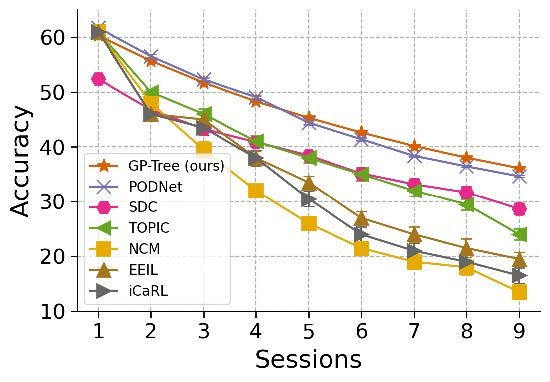
\includegraphics[width=0.5\linewidth]{images/achituve21d.jpg}
            \caption{Class-incremental few-shot learning results on mini-ImageNet. Test set accuracy averaged over 10 runs.}
            \label{fig:fig3}
        % \end{wrapfigure}
        
        \end{figure}
        The results for CUB are presented in Table \ref{tab:table3} and for mini-
        ImageNet in Figure \ref{fig:fig3}. On both datasets, we found the
        PyTorch implementation of ResNet-18 to be consistent with
        the results seen in (\textit{Tao et al., 2020}\cite{tao2020few}). We note that the results
        on mini-ImageNet could be improved by adapting the NN
        architecture for smaller images, but we kept the standard
        ResNet-18 for comparability with (\textit{Tao et al., 2020}\cite{tao2020few}).
        \\
        \\
        The comparison shows that while PODNet outperforms
        all other methods during the first sessions, our GP-Tree
        achieves the best accuracy in the remaining sessions (4-11
        in CUB and 5-9 in mini-ImageNet), where the challenges
        of avoiding catastrophic forgetting and learning from fewexamples
        become more difficult. We note that for CUB experiments
        the average SEM was $0.4$ and for mini-ImageNet
        it was $0.2$. These results indicate that using GPs can indeed
        handle incremental learning challenges better than current
        procedures, but there is still room for improvement in how it
        handles the base classes. We also note that when examining the accuracy per session across all sessions at each time step,
        we noticed that GP-Tree showed a higher accuracy on the
        base classes compared to novel classes. This is an expected
        outcome since the number of novel examples is small and
        the feature extractor is kept fixed during novel sessions. Improving
        the way GP-Tree handles novel sessions can further
        boost its performance. In supplementary Section D.2 we
        perform sensitivity analysis on the kernel function choice
        and the number of representative samples stored per class.
        We show that non-linear kernel functions are preferred over
        a linear kernel function. In supplementary Section D.3 we
        evaluate GP-Tree against baseline methods according to the
        average forgetting (\textit{Chaudhry et al., 2018}\cite{chaudhry2018riemannian}). We show that
        GP-Tree surpasses baseline methods on this aspect as well.

    \section{Conclusion}
    \label{sec:6}
    In this work, we showed how common Gaussian process
    classification methods struggle when facing classification
    tasks with a large number of classes. We presented our
    method, GP-tree, that scales with the number of classes and
    to large datasets. GP-tree uses the Pólya-Gamma augmentation
    and allows great flexibility in posterior inference that
    can be done either with a variational inference approach or
    a Gibbs sampling procedure. We further showed how GPTree
    can be naturally and successfully combined with DKL.
    Finally, we demonstrated how GP-tree can be adjusted to
    few-shot class-incremental learning challenges and showed
    how it achieves improved accuracy over current leading
    baseline methods. This indicates that Gaussian processes
    are a new and promising approach for this task.
    \section*{Acknowledgements}
    This study was funded by a grant to GC from the ISF (ISF 737/2018), and by an equipment
    grant to GC and Bar-Ilan University from the ISF (ISF 2332/18).

    \section*{BONUS}
        \textbf{Algorithm Example} (from \enquote{\textit{Massively Parallel and Asynchronous Tsetlin Machine Architecture Supporting
        Almost Constant-Time Scaling}})
    \label{sec:bonus}
        \begin{algorithm}[H]
        \SetAlgoNlRelativeSize{0}
        \caption{Decentralized updating of clause}
            \begin{algotithmic}
                
            \KwIn{Example pool $P$, clause $C_j$, positive polarity indicator $p_j \in \{0, 1\}$, batch size $b \in [1, \infty)$, voting margin $T \in [1, \infty)$, pattern specificity $s \in [1, \infty)$}
            \KwOut{Updated Clause: $C_j, p_j, P, b, T, s$}
            
            \For{$i = 1$ to $b$}{
                $(X_i, y_i, v_i) \leftarrow \text{ObtainTrainingExample}(P)$\;
                $v_i^c \leftarrow \text{clip}(v_i, -T, T)$\;
                $e = T - v_i^c \text{ if } y_i = 1 \text{ else } T + v_i^c$\;
                \If{$\text{rand()} \leq \frac{e}{2T}$}{
                    \If{$y_i \text{ xor } p_j$}{
                        $C_j \leftarrow \text{TypeIIFeedback}(X_i, C_j)$\;
                    }
                    \Else{
                        $C_j \leftarrow \text{TypeIFeedback}(X_i, C_j, s)$\;
                    }
                }
                $o_{ij} \leftarrow C_j(X_i)$\;
                $o_{ij}^* \leftarrow \text{ObtainPreviousClauseOutput}(i, j)$\;
                \If{$o_{ij} \neq o_{ij}^*$}{
                    $\text{AtomicAdd}(v_i, o_{ij} - o_{ij}^*)$\;
                    $\text{StorePreviousClauseOutput}(i, j, o_{ij})$\;
                }
            }
            \end{algotithmic}
        \end{algorithm}
% \\
%     \begin{algorithm}[H]
%         \SetAlgoNlRelativeSize{0}
%     \caption{An algorithm with caption}\label{alg:cap}
%     \begin{algorithmic}
%     \KwIn{Example pool $P$, clause $C_j$, positive polarity indicator $p_j \in \{0, 1\}$, batch size $b \in [1, \infty)$, voting margin $T \in [1, \infty)$, pattern specificity $s \in [1, \infty)$}
%     \Ensure $y = x^n$
%     \State $y \gets 1$
%     \State $X \gets x$
%     \State $N \gets n$
%     \While{$N \neq 0$}
%     \If{$N$ is even}
%         \State $X \gets X \times X$
%         \State $N \gets \frac{N}{2}$  \Comment{This is a comment}
%     \ElsIf{$N$ is odd}
%         \State $y \gets y \times X$
%         \State $N \gets N - 1$
%     \EndIf
%     \EndWhile
%     \end{algorithmic}
%     \end{algorithm}
\begin{multicols}{2}
    \bibliographystyle{ieeetr}
    \bibliography{references}   
\end{multicols}
\end{document}
